
\section{Qubits and Dirac Notation}

A classical \emph{bit} takes one of the two values $0$ and $1$. A quantum bit can be in a combination
of both.

\begin{definition}[Qubit, $n$-Qubit State]\label{def:qubit-0915}
    The state of one \textbf{qubit} is a unit vector in $\mathbb{C}^2$,
    \[\begin{pmatrix} \alpha \\ \beta \end{pmatrix}
        = \alpha \begin{pmatrix} 1 \\ 0 \end{pmatrix} + \beta \begin{pmatrix} 0 \\ 1 \end{pmatrix}
        = \alpha \ket{0} + \beta \ket{1},
        \qquad \abs{\alpha}^2 + \abs{\beta}^2 = 1,\]
    where $\ket{0} = \begin{pmatrix} 1 \\ 0 \end{pmatrix}$ and
    $\ket{1} = \begin{pmatrix} 0 \\ 1 \end{pmatrix}$ form the \textbf{computational basis}. The
    complex numbers $\alpha, \beta$ are the \textbf{amplitudes}. More generally, the state of $n$
    qubits is a unit vector in $\mathbb{C}^{2^n}$,
    \[\ket{\phi} = \sum_{x \in \set{0,1}^n} \alpha_x \ket{x},
        \qquad \sum_{x \in \set{0,1}^n} \abs{\alpha_x}^2 = 1,\]
    where $\ket{x}$ is the standard basis vector with a $1$ in the position indexed by the bit string
    $x$ (the $2^n$ strings are listed in increasing binary order) and $0$ elsewhere. Measuring the
    state gives the outcome $x$ with probability $\abs{\alpha_x}^2$.
\end{definition}

\paragraph{Two qubits.} The state of two qubits has four amplitudes:
$(\alpha, \beta, \gamma, \delta)^T = \alpha \ket{00} + \beta \ket{01} + \gamma \ket{10} + \delta \ket{11}$
with $\abs{\alpha}^2 + \abs{\beta}^2 + \abs{\gamma}^2 + \abs{\delta}^2 = 1$, where
$\ket{00}, \ket{01}, \ket{10}, \ket{11}$ are the four standard basis column vectors of
$\mathbb{C}^4$, in this order.

\needspace{9\baselineskip} % keep the exercise and the start of its solution on one page
\begin{exercisebox}
\begin{exercise}\label{ex:basis-0915}
    What is the third entry of the column vector $\ket{00}$?
\end{exercise}
\tcblower
\begin{wsolution}
    It is $0$. The third entry is the amplitude of $\ket{10}$, and
    $\ket{00} = 1 \cdot \ket{00} + 0 \cdot \ket{01} + 0 \cdot \ket{10} + 0 \cdot \ket{11}$, so
    $\ket{00} = (1, 0, 0, 0)^T$.
\end{wsolution}
\end{exercisebox}

Writing a column vector as a combination of the kets $\ket{x}$ is \emph{Dirac notation}. The state
$\frac{1}{\sqrt{2}} \ket{0000} + \frac{1}{\sqrt{2}} \ket{1111}$ of four qubits is a column vector
with $2^4 = 16$ entries: $\sfrac{1}{\sqrt{2}}$ in the first and in the last position and $0$ in the
other fourteen.

\subsection{Kets, Bras and the Dagger}

A \emph{ket} $\ket{\phi}$ is a column vector. The corresponding \emph{bra} is the row vector
$\bra{\phi} = \left(\ket{\phi}\right)^\dagger$, where $\dagger$ (``dagger'') is the
\emph{conjugate transpose}: transpose and replace every entry by its complex conjugate. For
$\ket{\phi} = \begin{pmatrix} \alpha \\ \beta \end{pmatrix}$ we get
$\bra{\phi} = \begin{pmatrix} \overline{\alpha} & \overline{\beta} \end{pmatrix}$. The dagger equals
the inverse only for unitary matrices (\cref{def:unitary-0915}).

A bra times a ket is a number, the \emph{inner product}, and it gives the (Euclidean) norm. For
$\ket{x}, \ket{y} \in \mathbb{C}^n$ with entries $x_i$, $y_i$,
\[\braket{x}{y} = \bra{x} \ket{y} = \sum_{i=1}^{n} \overline{x_i} \, y_i,
    \qquad
    \norm{\ket{y}}^2 = \braket{y}{y} = \sum_{i=1}^{n} \abs{y_i}^2.\]
The inner product is linear in the second argument and conjugate-linear in the first, and
$\braket{y}{x} = \overline{\braket{x}{y}}$. We use two rules for the dagger:
$(A^\dagger)^\dagger = A$, and $(AB)^\dagger = B^\dagger A^\dagger$ for matrices $A$, $B$ whose
product is defined. So $\left(U \ket{x}\right)^\dagger = \bra{x} U^\dagger$.

\section{Unitary Matrices}

\begin{definition}[Unitary Matrix]\label{def:unitary-0915}
    An $n \times n$ complex matrix $U$ is \textbf{unitary} if $U^\dagger U = I$.
\end{definition}

\begin{exercisebox}
\begin{exercise}\label{ex:unitary-0915}\label{thm:unitary-0915}
    Let $U$ be an $n \times n$ complex matrix. Show that $\norm{U \ket{x}} = \norm{\ket{x}}$ for all
    $\ket{x} \in \mathbb{C}^n$ if and only if $U$ is unitary ($U^\dagger U = I$).
\end{exercise}
\tcblower
\begin{proof}
    \emph{Unitary implies norm preserving.} If $U^\dagger U = I$, then for every $\ket{x}$,
    $\norm{U \ket{x}}^2 = \left(U \ket{x}\right)^\dagger U \ket{x} = \bra{x} U^\dagger U \ket{x}
        = \braket{x}{x} = \norm{\ket{x}}^2$.
    Norms are non-negative, so $\norm{U \ket{x}} = \norm{\ket{x}}$.

    \emph{Norm preserving implies unitary.} Let $M = U^\dagger U - I$. Then $M^\dagger = M$, and for
    every $\ket{x}$,
    \[\bra{x} M \ket{x} = \norm{U \ket{x}}^2 - \norm{\ket{x}}^2 = 0.\]
    Let $z = \bra{x} M \ket{y}$, so that $\bra{y} M \ket{x} = \overline{z}$. Applying the last
    equation to $\ket{x} + \ket{y}$ and to $\ket{x} + i \ket{y}$ gives
    \[0 = z + \overline{z} = 2 \operatorname{Re} z,
        \qquad
        0 = i \left(z - \overline{z}\right) = -2 \operatorname{Im} z.\]
    So $\bra{x} M \ket{y} = 0$ for all $\ket{x}, \ket{y}$. For the basis vectors $e_j$ and $e_k$ this
    says $M_{jk} = 0$. So $M = 0$, which is $U^\dagger U = I$.
\end{proof}
\end{exercisebox}

\paragraph{Remark.} A quantum gate is a linear map that sends every state (every unit vector) to a
state. Every vector is a multiple of a unit vector, so such a map preserves the norm of all vectors.
By \cref{thm:unitary-0915} it is unitary. Conversely, every unitary matrix maps states to states.

\section{Quantum Circuits and One-Qubit Gates}

A \emph{quantum circuit} is drawn with one horizontal wire per qubit. Time runs from left to right,
and a box on a wire is a gate (a unitary matrix) applied to that qubit (\cref{fig:xh-0915}).

\paragraph{Columns of a matrix.} Let $A$ be an $m \times n$ matrix with columns $a_1, \dots, a_n$,
and let $x = (x_1, \dots, x_n)^T$. Then $A x = x_1 a_1 + x_2 a_2 + \dots + x_n a_n$. So
$A e_j = a_j$: \emph{the $\nth{j}$ column of a gate's matrix is the image of the $\nth{j}$ basis
state}.

\paragraph{The $X$ gate.} The \emph{Pauli $X$ gate} is the quantum NOT gate, with
$X \ket{0} = \ket{1}$ and $X \ket{1} = \ket{0}$. By linearity,
\[X = \sigma_x = \begin{pmatrix} 0 & 1 \\ 1 & 0 \end{pmatrix},
    \qquad
    X \left(\alpha \ket{0} + \beta \ket{1}\right) = \alpha \ket{1} + \beta \ket{0}.\]

\begin{definition}[Hadamard Gate]\label{def:hadamard-0915}
    The \textbf{Hadamard gate} $H$ is the one-qubit gate with
    \begin{equation}\label{eq:hadamard-0915}
        H \ket{0} = \frac{1}{\sqrt{2}}\left(\ket{0} + \ket{1}\right),
        \qquad
        H \ket{1} = \frac{1}{\sqrt{2}}\left(\ket{0} - \ket{1}\right),
        \qquad
        H = \frac{1}{\sqrt{2}} \begin{pmatrix} 1 & 1 \\ 1 & -1 \end{pmatrix}.
    \end{equation}
\end{definition}

Both $H \ket{0}$ and $H \ket{1}$ are equal superpositions: measuring gives $0$ and $1$ with
probability $\sfrac{1}{2}$ each.

\begin{lemma}[Hadamard Twice Is the Identity]\label{lem:hh-0915}
    $H^2 = I$. So $H$ is unitary, and
    \[H \, \frac{1}{\sqrt{2}}\left(\ket{0} + \ket{1}\right) = \ket{0},
        \qquad
        H \, \frac{1}{\sqrt{2}}\left(\ket{0} - \ket{1}\right) = \ket{1}.\]
\end{lemma}

\begin{proof}
    The diagonal entries of $H^2$ are $\frac{1}{2}(1 \cdot 1 + 1 \cdot 1) = 1$
    and $\frac{1}{2}(1 \cdot 1 + (-1)(-1)) = 1$, and both off-diagonal entries are
    $\frac{1}{2}(1 \cdot 1 + 1 \cdot (-1)) = 0$, so $H^2 = I$.
    $H$ is real and symmetric, so $H^\dagger = H$ and $H^\dagger H = H^2 = I$.
    By \cref{eq:hadamard-0915}, the two states in the statement are $H \ket{0}$ and $H \ket{1}$, and
    $H H \ket{0} = \ket{0}$, $H H \ket{1} = \ket{1}$.
\end{proof}

\begin{figure}[ht]
    \centering
    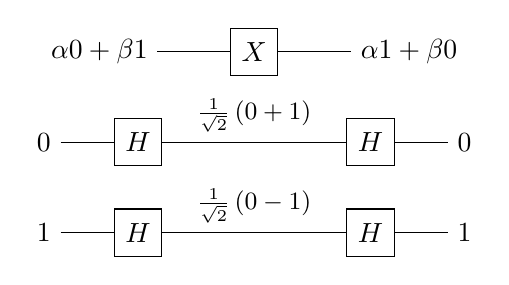
\begin{tikzpicture}[scale=0.82, 
            gate/.style={draw, fill=white, minimum size=6mm, inner sep=1pt},
        ]
        \draw (1.5,2.8) -- (4.5,2.8);
        \node[left] at (1.5,2.8) {$\alpha\ket{0} + \beta\ket{1}$};
        \node[gate] at (3,2.8) {$X$};
        \node[right] at (4.5,2.8) {$\alpha\ket{1} + \beta\ket{0}$};
        \draw (0,1.4) -- (6,1.4);
        \node[left] at (0,1.4) {$\ket{0}$};
        \node[gate] at (1.2,1.4) {$H$};
        \node[above] at (3,1.4) {\small $\frac{1}{\sqrt{2}}\left(\ket{0} + \ket{1}\right)$};
        \node[gate] at (4.8,1.4) {$H$};
        \node[right] at (6,1.4) {$\ket{0}$};
        \draw (0,0) -- (6,0);
        \node[left] at (0,0) {$\ket{1}$};
        \node[gate] at (1.2,0) {$H$};
        \node[above] at (3,0) {\small $\frac{1}{\sqrt{2}}\left(\ket{0} - \ket{1}\right)$};
        \node[gate] at (4.8,0) {$H$};
        \node[right] at (6,0) {$\ket{1}$};
    \end{tikzpicture}
    \caption{Top: the $X$ gate. Below: the Hadamard gate applied twice (\cref{lem:hh-0915}).}
    \label{fig:xh-0915}
\end{figure}

\section{The CNOT Gate}

\begin{definition}[CNOT Gate]\label{def:cnot-0915}
    The \textbf{controlled-NOT gate} (CNOT) is the two-qubit gate that maps the basis states by
    \[\ket{a} \ket{b} \longmapsto \ket{a} \ket{b \oplus a}, \qquad a, b \in \set{0,1},\]
    where $\oplus$ is XOR (addition modulo $2$). The first qubit $\ket{a}$ is the \textbf{control}
    qubit and is left unchanged. The second qubit $\ket{b}$ is the \textbf{target} qubit and is flipped
    exactly when $a = 1$. See \cref{fig:cnot-0915}.
\end{definition}

\begin{figure}[ht]
    \centering
    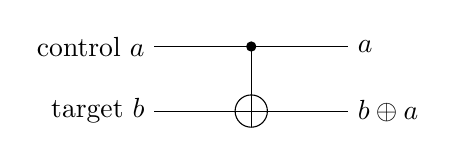
\begin{tikzpicture}[scale=0.82]
        \draw (0,1) -- (3,1);
        \draw (0,0) -- (3,0);
        \node[left] at (0,1) {control $\ket{a}$};
        \node[left] at (0,0) {target $\ket{b}$};
        \filldraw (1.5,1) circle (2pt);
        \draw (1.5,1) -- (1.5,-0.25);
        \draw (1.5,0) circle (0.25);
        \node[right] at (3,1) {$\ket{a}$};
        \node[right] at (3,0) {$\ket{b \oplus a}$};
    \end{tikzpicture}
    \caption{The CNOT gate: a filled dot on the control qubit and $\oplus$ on the target qubit.}
    \label{fig:cnot-0915}
\end{figure}

\begin{lemma}[Matrix of the CNOT Gate]\label{lem:cnot-0915}
    The matrix of the CNOT gate, with rows and columns indexed by $00, 01, 10, 11$, is the
    permutation matrix
    \[U_{\mathrm{CNOT}} = \begin{pmatrix}
            1 & 0 & 0 & 0 \\
            0 & 1 & 0 & 0 \\
            0 & 0 & 0 & 1 \\
            0 & 0 & 1 & 0
        \end{pmatrix}.\]
    It is unitary.
\end{lemma}

\begin{proof}
    The columns of the matrix of a gate are the images of the basis states. By \cref{def:cnot-0915},
    $\ket{00}, \ket{01}, \ket{10}, \ket{11}$ go to $\ket{00}, \ket{01}, \ket{11}, \ket{10}$, which
    are the four columns of $U_{\mathrm{CNOT}}$ in this order. They are the four standard basis
    vectors, each once, so $U_{\mathrm{CNOT}}$ is a \emph{permutation matrix}.

    A permutation matrix $P$ is unitary: the $(j, k)$ entry of $P^T P$ is the inner product of the
    $\nth{j}$ and the $\nth{k}$ column of $P$, which is $1$ if $j = k$ and $0$ otherwise. So
    $P^\dagger P = P^T P = I$.
\end{proof}

In block form, $U_{\mathrm{CNOT}} = \begin{pmatrix} I & 0 \\ 0 & X \end{pmatrix}$. If the control is
$0$ nothing happens, and if it is $1$ the gate $X$ is applied to the target.

\subsection{Classical Gates Are Not Reversible}

By \cref{thm:unitary-0915} and the remark after it, every quantum gate is unitary, so applying
$U^\dagger$ undoes it. Classical gates that take two bits to one bit, such as AND, OR and XOR, are
\emph{not bijective}, so \emph{not reversible}, and so \emph{not unitary}.

\begin{lemma}[XOR Is Not Reversible]\label{lem:xor-0915}
    The classical gate $\mathrm{XOR} \colon (a, b) \mapsto a \oplus b$ is not injective, so its
    input cannot be recovered from its output. The linear map
    $T \colon \mathbb{C}^4 \to \mathbb{C}^2$ with $T \ket{a b} = \ket{a \oplus b}$ does not preserve
    norms, so it is not unitary. The same holds for AND and OR.
\end{lemma}

\begin{proof}
    $\mathrm{XOR}(0,0) = 0 = \mathrm{XOR}(1,1)$, and
    $T\left(\ket{00} - \ket{11}\right) = \ket{0} - \ket{0} = 0$ although
    $\norm{\ket{00} - \ket{11}} = \sqrt{2}$. For AND use the inputs $00$ and $01$, and for OR use
    $01$ and $11$.
\end{proof}

\section{Tensor Products and Entanglement}

\begin{definition}[Tensor Product]\label{def:tensor-0915}
    Let $A = (a_{ij})$ be an $m \times n$ matrix and let $B$ be a $p \times q$ matrix. The
    \textbf{tensor product} (Kronecker product) $A \otimes B$ is the $mp \times nq$ block matrix
    \[A \otimes B = \begin{pmatrix}
            a_{11} B & a_{12} B & \cdots & a_{1n} B \\
            a_{21} B & a_{22} B & \cdots & a_{2n} B \\
            \vdots   &          &        & \vdots   \\
            a_{m1} B & a_{m2} B & \cdots & a_{mn} B
        \end{pmatrix}.\]
    Column vectors are matrices with one column, so
    \[\begin{pmatrix} \alpha \\ \beta \end{pmatrix} \otimes \begin{pmatrix} \gamma \\ \delta \end{pmatrix}
        = \begin{pmatrix} \alpha\gamma \\ \alpha\delta \\ \beta\gamma \\ \beta\delta \end{pmatrix}.\]
\end{definition}

For example, $\ket{1} \otimes \ket{0} = (0, 0, 1, 0)^T = \ket{10}$, and
in general $\ket{a} \ket{b} = \ket{a} \otimes \ket{b} = \ket{a b}$ for $a, b \in \set{0,1}$. In terms
of kets, $\left(\alpha \ket{0} + \beta \ket{1}\right) \otimes \left(\gamma \ket{0} + \delta \ket{1}\right)
    = \alpha\gamma \ket{00} + \alpha\delta \ket{01} + \beta\gamma \ket{10} + \beta\delta \ket{11}$.
If $A$ is applied to the first qubit and $B$ to the second, the two-qubit gate is $A \otimes B$, and
\begin{equation}\label{eq:mixed-0915}
    (A \otimes B)\left(\ket{x} \otimes \ket{y}\right) = A \ket{x} \otimes B \ket{y}.
\end{equation}
If $x_1, \dots, x_n$ are the entries of $\ket{x}$, then $\ket{x} \otimes \ket{y}$ consists of
the blocks $x_1 \ket{y}, \dots, x_n \ket{y}$. So the $\nth{i}$ block of the left-hand side is
$\sum_{j} a_{ij} B \left(x_j \ket{y}\right) = \left(\sum_j a_{ij} x_j\right) B \ket{y}$, which is the
$\nth{i}$ block of the right-hand side.

\begin{definition}[Product State, Entangled State]
    A two-qubit state $\ket{\psi}$ is a \textbf{product state} if
    $\ket{\psi} = \ket{\phi_1} \otimes \ket{\phi_2}$ for some one-qubit states $\ket{\phi_1}$,
    $\ket{\phi_2}$. Otherwise $\ket{\psi}$ is \textbf{entangled}.
\end{definition}

\needspace{9\baselineskip} % keep the exercise and the start of its solution on one page
\begin{exercisebox}
\begin{exercise}\label{ex:bell-0915}\label{thm:bell-0915}
    Show that the \emph{Bell state} $\frac{1}{\sqrt{2}} \ket{00} + \frac{1}{\sqrt{2}} \ket{11}$ is
    entangled: there are no vectors $\ket{\phi_1}, \ket{\phi_2} \in \mathbb{C}^2$ with
    \[\frac{1}{\sqrt{2}} \ket{00} + \frac{1}{\sqrt{2}} \ket{11} = \ket{\phi_1} \otimes \ket{\phi_2}.\]
\end{exercise}
\tcblower
\begin{proof}
    Suppose there are, and write $\ket{\phi_1} = \begin{pmatrix} \alpha \\ \beta \end{pmatrix}$ and
    $\ket{\phi_2} = \begin{pmatrix} \gamma \\ \delta \end{pmatrix}$. By \cref{def:tensor-0915},
    comparing the four entries of the two sides gives $\alpha\gamma = \sfrac{1}{\sqrt{2}}$,
    $\alpha\delta = 0$, $\beta\gamma = 0$ and $\beta\delta = \sfrac{1}{\sqrt{2}}$.
    From $\alpha\delta = 0$ we get $\alpha = 0$ or $\delta = 0$. If $\alpha = 0$ then
    $\alpha\gamma = 0 \neq \sfrac{1}{\sqrt{2}}$, and if $\delta = 0$ then
    $\beta\delta = 0 \neq \sfrac{1}{\sqrt{2}}$. Both cases are contradictions.
\end{proof}
\end{exercisebox}
